% !TeX program = lualatex
% SHR Converter 0.0.2 - user and technical manual. Generated by tools/build_manual.py; edit that, not this.
\documentclass[11pt,a4paper]{article}
\usepackage{fontspec}
\usepackage[margin=2.2cm]{geometry}
\usepackage{amsmath,amssymb}
\usepackage{booktabs,longtable,tabularx,array}
\usepackage{graphicx}
\usepackage{xcolor}
\usepackage{caption}
\usepackage{enumitem}
\usepackage[hidelinks,bookmarksnumbered,bookmarksopen,bookmarksopenlevel=2,
            pdftitle={SHR Converter 0.0.2 - Manual},
            pdfauthor={William W. Wallace},
            pdfsubject={Signal Hound Spike .shr to CSV and Veusz .vszh5},
            pdfkeywords={Signal Hound, Spike, SM200C, SHR, CSV, Veusz, vszh5, spectrogram}]{hyperref}
\usepackage{bookmark}
\urlstyle{same}
\setlength{\LTcapwidth}{\linewidth}
\setlength{\emergencystretch}{3em}
\captionsetup[longtable]{justification=centering}
\newcommand{\code}[1]{\texttt{#1}}
\title{SHR Converter 0.0.2\\[4pt]\large Signal Hound Spike \code{.shr} recordings to CSV and native Veusz documents\\
User and technical manual}
\author{William W. Wallace\\NRAO/GBO\\\code{wwallace@nrao.edu}}
\date{2026-10-28}
\begin{document}
\maketitle
\begin{center}
\begin{tabular}{ll}
\toprule
Program & Version\\
\midrule
\code{shr\_converter.py} (launcher) & 0.0.2\\
\code{shr\_converter\_gui.py} & 0.0.2\\
\code{shr\_converter\_core.py} & 0.0.2\\
\code{shr\_reader.py} (reader) & 0.0.1\\
\code{vszh5\_writer.py} & 0.0.21\\
\bottomrule
\end{tabular}
\end{center}
\tableofcontents
\clearpage

\section{Overview}
Spike, Signal Hound's analyzer software, records sweeps to \code{.shr} files: a 472-byte file header, then
per sweep a 48-byte sweep header (time stamp, GPS latitude/longitude/altitude, ADC-overflow flag) and the
amplitudes as 32-bit floats \cite{r1},\cite{r2}. The SHR Converter reads these files with its own reader,
\code{shr\_reader}, written from the definition in Signal Hound's SDK (\code{shr\_parse.h}) \cite{r1} and
needing only NumPy. It writes CSV tables and a native Veusz document (\code{.vszh5}) through the author's
\code{vszh5\_writer} \cite{r3}, optionally rendered by Veusz \cite{r14} to a bookmarked PDF and PNGs.
Everything is streamed in blocks, so memory is set by a RAM budget and not by the file, and the blocks run in
parallel worker processes, with the numerical part on the GPU when CuPy is present.

\subsection{What is new in 0.0.2}
\begin{itemize}[nosep]
\item \textbf{Own reader.} Version 0.0.1 used py-shr-parser 1.0.0 \cite{r10}, which stops with
      \code{ValueError: 2 is not a valid ShrVideoDetector} on SM200C recordings from current Spike releases:
      their \code{detector} field holds code 2, which the SDK's enumeration does not list. \code{shr\_reader}
      keeps every raw code, labels it with a stated confidence and never refuses a file for an unknown value
      (Section~\ref{sec:format}).
\item \textbf{Multi-file recordings} (Spike~3.9.7 \cite{r9}) are joined into one recording
      (Section~\ref{sec:join}).
\item \textbf{CSV time decimation}: N sweeps per CSV row, by peak hold, power mean or minimum hold
      (Section~\ref{sec:decimate}).
\item \textbf{vszh5\_writer 0.0.21}: no false blank spectrogram rows from millisecond time-stamp
      jitter (Section~\ref{sec:grid}).
\item GHz axes above 10~GHz, short page titles, wrapped header page; detector shown on the statistics page.
\end{itemize}

\section{Installation}
\begin{enumerate}[nosep]
\item \code{mamba env create -f environment.yml} --- Python 3.12; pip installs \code{requirements.txt}
      (NumPy, h5py, Qt.py, PySide6, pyqtgraph, psutil, pypdf).
\item \code{mamba activate shr-converter}
\item Optional: \code{mamba install -c conda-forge veusz} (or the Veusz installer) to open and render;
      \code{mamba install -c conda-forge cupy} for an NVIDIA GPU.
\item \code{python shr\_converter.py --selftest --gui-smoke} --- 39 reader checks, 58 engine checks
      and 12 GUI checks.
\item \code{python shr\_converter.py} starts the GUI. On Windows: \code{create\_environment.bat} once,
      then \code{run\_shr\_converter.bat} (files may be dropped on it) and \code{run\_selftest.bat}.
\item \code{python shr\_converter.py --reader file.shr} prints a file's header, enumerations, notes and
      amplitude grid without converting anything (\code{--json}, \code{--group}, \code{--grid}).
\end{enumerate}
The launcher imports nothing heavy at its top level: worker processes started with \emph{spawn} re-run the
main script's top level, and this keeps Qt (about 50~MB per process) out of them.

\section{\texorpdfstring{The \code{.shr} format and \code{shr\_reader}}{The .shr format and shr\_reader}}\label{sec:format}
\subsection{Byte layout}
All fields are little-endian and packed (no padding) \cite{r1}. A file of $S$ bytes with $n$ bins per sweep
holds
\begin{equation}
N_\mathrm{complete}=\left\lfloor\frac{S-\code{dataOffset}}{48+4n}\right\rfloor
\end{equation}
complete sweep records of $48+4n$ bytes each; the SM200C sample ($n=8384$) has records of 33\,584 bytes. The
reader parses the header with one \code{struct} call and maps the records as a NumPy structured array, so a
block of sweeps is one slice of a memory map and no Python loop runs per sweep.
\begin{longtable}{rp{3.4cm}p{4.2cm}l}
\caption{File header (472 bytes), generated from shr\_reader.HEADER\_LAYOUT.}\\
\toprule
\textbf{Offset} & \textbf{SDK name} & \textbf{shr\_reader name} & \textbf{C type}\\
\midrule
\endhead
0 & \texttt{signature} & \texttt{signature} & uint16\\
2 & \texttt{version} & \texttt{version} & uint16\\
4 & \texttt{reserved1} & \texttt{reserved1} & uint32\\
8 & \texttt{dataOffset} & \texttt{data\_\allowbreak{}offset} & uint64\\
16 & \texttt{sweepCount} & \texttt{sweep\_\allowbreak{}count} & uint32\\
20 & \texttt{sweepLength} & \texttt{sweep\_\allowbreak{}length} & uint32\\
24 & \texttt{firstBinFreqHz} & \texttt{first\_\allowbreak{}bin\_\allowbreak{}freq\_\allowbreak{}hz} & double\\
32 & \texttt{binSizeHz} & \texttt{bin\_\allowbreak{}size\_\allowbreak{}hz} & double\\
40 & \texttt{title} & \texttt{title\_\allowbreak{}raw} & uint16[128]\\
296 & \texttt{centerFreqHz} & \texttt{center\_\allowbreak{}freq\_\allowbreak{}hz} & double\\
304 & \texttt{spanHz} & \texttt{span\_\allowbreak{}hz} & double\\
312 & \texttt{rbwHz} & \texttt{rbw\_\allowbreak{}hz} & double\\
320 & \texttt{vbwHz} & \texttt{vbw\_\allowbreak{}hz} & double\\
328 & \texttt{refLevel} & \texttt{ref\_\allowbreak{}level} & float\\
332 & \texttt{refScale} & \texttt{ref\_\allowbreak{}scale} & uint32\\
336 & \texttt{div} & \texttt{div} & float\\
340 & \texttt{window} & \texttt{window} & uint32\\
344 & \texttt{attenuation} & \texttt{attenuation} & int32\\
348 & \texttt{gain} & \texttt{gain} & int32\\
352 & \texttt{detector} & \texttt{detector} & int32\\
356 & \texttt{processingUnits} & \texttt{processing\_\allowbreak{}units} & int32\\
360 & \texttt{windowBandwidth} & \texttt{window\_\allowbreak{}bandwidth} & double\\
368 & \texttt{decimationType} & \texttt{decimation\_\allowbreak{}type} & int32\\
372 & \texttt{decimationDetector} & \texttt{decimation\_\allowbreak{}detector} & int32\\
376 & \texttt{decimationCount} & \texttt{decimation\_\allowbreak{}count} & int32\\
380 & \texttt{decimationTimeMs} & \texttt{decimation\_\allowbreak{}time\_\allowbreak{}ms} & int32\\
384 & \texttt{channelizeEnabled} & \texttt{channelize\_\allowbreak{}enabled} & int32\\
388 & \texttt{channelOutputUnits} & \texttt{channel\_\allowbreak{}output\_\allowbreak{}units} & int32\\
392 & \texttt{channelCenterHz} & \texttt{channel\_\allowbreak{}center\_\allowbreak{}hz} & double\\
400 & \texttt{channelWidthHz} & \texttt{channel\_\allowbreak{}width\_\allowbreak{}hz} & double\\
408 & \texttt{reserved2} & \texttt{reserved2} & uint8[64]\\
\bottomrule
\end{longtable}
\begin{longtable}{rp{3.4cm}p{4.2cm}l}
\caption{One sweep record: 48-byte sweep header, then the amplitudes.}\\
\toprule
\textbf{Offset} & \textbf{SDK name} & \textbf{shr\_reader name} & \textbf{C type}\\
\midrule
\endhead
0 & \texttt{timestamp} & \texttt{timestamp\_\allowbreak{}ms} & uint64\\
8 & \texttt{latitude} & \texttt{latitude} & double\\
16 & \texttt{longitude} & \texttt{longitude} & double\\
24 & \texttt{altitude} & \texttt{altitude\_\allowbreak{}m} & double\\
32 & \texttt{adcOverflow} & \texttt{adc\_\allowbreak{}overflow} & uint8\\
33 & \texttt{reserved[15]} & \texttt{reserved} & uint8[15]\\
48 & sweep data & \texttt{amplitude} & float32 x sweepLength\\
\bottomrule
\end{longtable}

\subsection{Enumerations and their confidence}
Every enumerated field is stored as its raw integer. Labels carry a confidence: \emph{documented} (in
\code{shr\_parse.h}), \emph{inferred} (from data, see below) or \emph{unverified} (by analogy, no file seen).
Any other code is shown as ``unknown (code $c$)'' and becomes a note; it never stops a conversion.
\begin{longtable}{p{4.2cm}rp{4.4cm}l}
\caption{Enumerations, generated from shr\_reader.ENUM\_FIELDS.}\\
\toprule
\textbf{Field} & \textbf{Code} & \textbf{Label} & \textbf{Confidence}\\
\midrule
\endhead
\texttt{ref\_\allowbreak{}scale} & 0 & dBm & documented\\
\texttt{ref\_\allowbreak{}scale} & 1 & mV & documented\\
\texttt{window} & 0 & Nuttall & documented\\
\texttt{window} & 1 & Flattop & documented\\
\texttt{window} & 2 & Gaussian & documented\\
\texttt{detector} & 0 & MinMax & documented\\
\texttt{detector} & 1 & Average & documented\\
\texttt{detector} & 2 & Max & inferred\\
\texttt{detector} & 3 & Min & unverified\\
\texttt{processing\_\allowbreak{}units} & 0 & Log & documented\\
\texttt{processing\_\allowbreak{}units} & 1 & Voltage & documented\\
\texttt{processing\_\allowbreak{}units} & 2 & Power & documented\\
\texttt{processing\_\allowbreak{}units} & 3 & Sample & documented\\
\texttt{decimation\_\allowbreak{}type} & 0 & Time & documented\\
\texttt{decimation\_\allowbreak{}type} & 1 & Count & documented\\
\texttt{decimation\_\allowbreak{}detector} & 0 & Average & documented\\
\texttt{decimation\_\allowbreak{}detector} & 1 & Max & documented\\
\texttt{channel\_\allowbreak{}output\_\allowbreak{}units} & 0 & dBm & documented\\
\texttt{channel\_\allowbreak{}output\_\allowbreak{}units} & 1 & dBm/Hz & documented\\
\bottomrule
\end{longtable}

\subsection{Why detector code 2 is read as Max}
Spike~3.5.7 added max and min detectors \cite{r9}; the SDK lists only 0~=~MinMax and 1~=~Average
\cite{r1}. Two independent tests on the SM200C sample (460 sweeps $\times$ 8384 bins, detector~2) point to
Max:
\begin{enumerate}[nosep]
\item \textbf{Amplitude grid.} For min/max processing the SM series converts each FFT to 0.01~dB resolution
      \cite{r11}. All 4\,999 distinct values of the sample satisfy
      \begin{equation}x=0.01\,k+0.00824~\mathrm{dB},\qquad k\in\mathbb Z,\end{equation}
      with a largest residual of $7.3\times10^{-6}$~dB (float32 precision). An average detector gives
      continuous values, so the file came through the min/max path.
\item \textbf{Noise shape.} In a noise-only bin the power of one FFT is exponential (unit mean). The maximum
      $M$ of $K$ FFTs has
      \begin{equation}
      P(M\le x)=\left(1-e^{-x}\right)^K,\qquad \mathrm E[M]=H_K=\sum_{k=1}^{K}\frac1k\approx\ln K+\gamma ,
      \end{equation}
      and $M-\ln K$ tends to the Gumbel distribution (standard deviation $\pi/\sqrt6\approx1.283$, skewness
      $+1.14$). With $Y=10\log_{10}M$ and $\mathrm dY=\frac{10}{\ln10}\frac{\mathrm dM}{M}$,
      \begin{equation}
      \sigma_Y\approx\frac{10}{\ln 10}\,\frac{\pi/\sqrt6}{\ln K+\gamma}
      =\frac{4.343\times1.283}{6.238+0.577}=0.82~\mathrm{dB}\quad(K=512),
      \end{equation}
      skewed to the right. The sample's noise bins give $\sigma=0.745$~dB and skewness $+0.51$, against
      0.77~dB and $+0.50$ simulated for the max of 512 FFTs. A minimum gives $\sigma_Y=5.57$~dB for every $K$,
      and a power average gives $\sigma_Y\approx4.343/\sqrt K$ with negative skew; neither fits.
\end{enumerate}
The full analysis is in \code{docs/design/SM200C\_SHR\_PARSER\_BRIEF\_0.0.1.md}. Code~3~=~Min is assumed by
analogy, and what a MinMax (code~0) file stores is not known; both are among the questions to Signal Hound
(\code{docs/SignalHound\_support\_letter\_2026-10-28.md}).
\begin{figure}[htbp]\centering
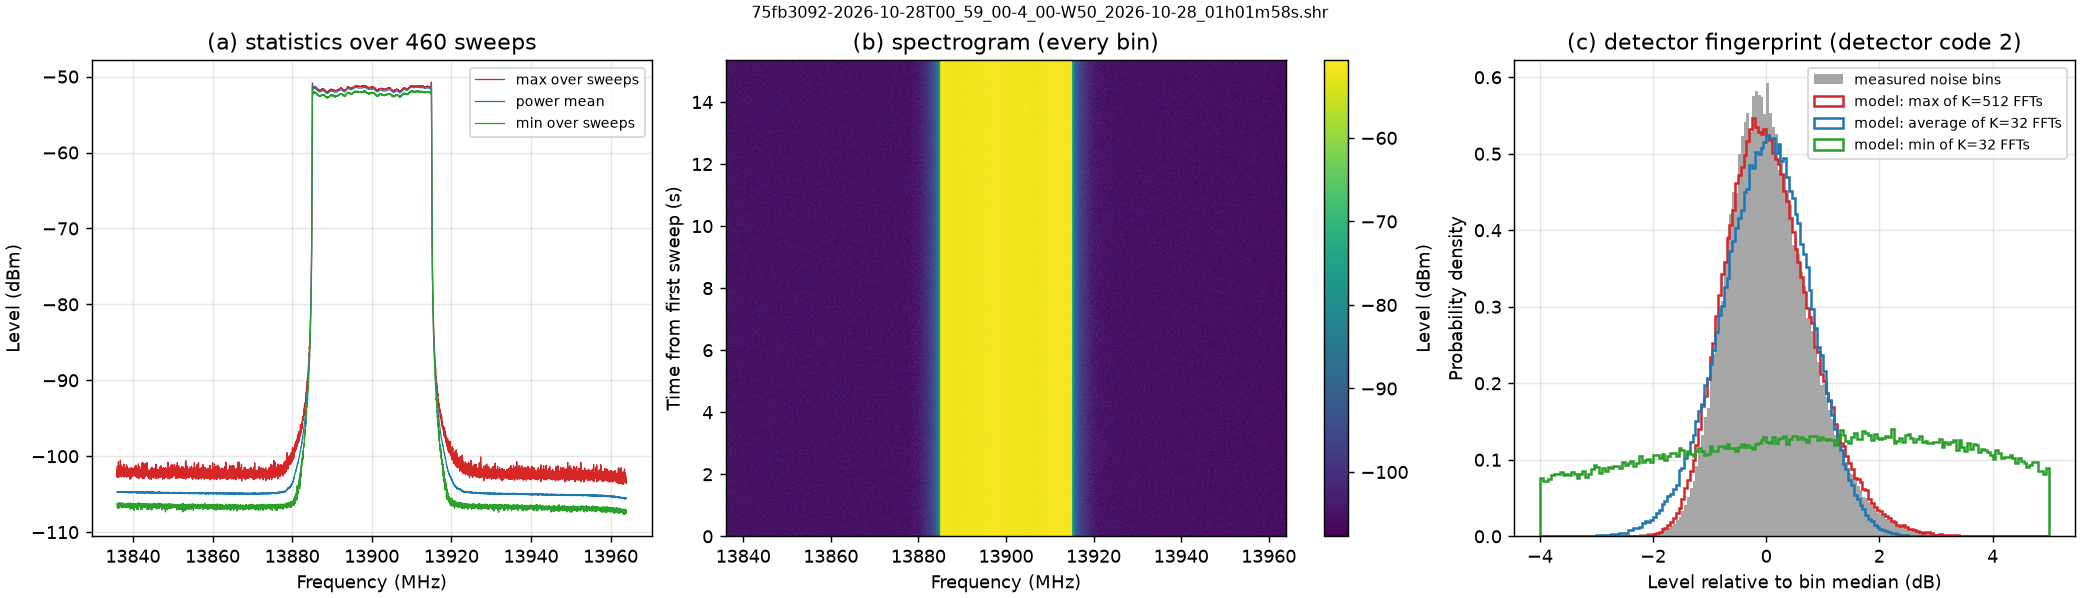
\includegraphics[width=\linewidth]{design/figures/sm200c_sample_analysis.png}
\caption{SM200C sample: (a) max, power mean and min over 460 sweeps; (b) spectrogram; (c) noise distribution against detector models (max of K = 512 FFTs fits).}
\end{figure}

\subsection{Amplitude-grid detection}
\code{detect\_amplitude\_grid} scales the distinct values by the step $q=0.01$~dB and takes their common
fractional part as a circular mean,
\begin{equation}
\phi=\frac{1}{2\pi}\arg\Big(\frac1m\sum_{j=1}^{m}e^{2\pi i\,(x_j/q\bmod 1)}\Big)\bmod 1,
\qquad r_j=\Big|\Big(\frac{x_j}{q}-\phi+\tfrac12\Big)\bmod 1-\tfrac12\Big|\,q ,
\end{equation}
so an offset near 0 (values just below and just above whole steps) is not averaged to $q/2$. The values are on
the grid when $\max_j r_j<5\times10^{-4}$~dB and there are at least 16 distinct values. The converter then
notes that fixed-decimal CSV output moves values by up to half a step; lossless output is unaffected.

\subsection{Validation and salvage}
\begin{itemize}[nosep]
\item Signature other than \code{0xAA10}, impossible sizes or a header shorter than 472 bytes: \code{ShrFormatError}.
\item Version above 2: read with the version-2 layout, with a note.
      \code{dataOffset} larger than 472 is honoured.
\item \code{sweepCount} = 0 (recording not closed): the complete sweeps present are read.
\item \code{sweepCount} larger than $N_\mathrm{complete}$ (cut short): $N_\mathrm{complete}$ sweeps are read.
\item Complete sweeps beyond \code{sweepCount}, and trailing bytes after the last complete sweep: ignored,
      with a note.
\item Every note reaches the GUI, the log, \code{\_header.csv} and the header page.
\end{itemize}

\subsection{Using the reader from Python}
\begin{itemize}[nosep]
\item \code{open\_recording(path or list)} returns a \code{ShrFile} or, for several files, a
      \code{ShrFileSet}; both have \code{n\_sweeps}, \code{n\_bins}, \code{header},
      \code{frequencies\_hz()}, \code{read(start, stop, step, col0, col1)} (a \code{SweepBlock} of
      amplitudes, time stamps, GPS and overflow), \code{get\_sweep(k)}, \code{iter\_blocks()} and
      \code{close()}.
\item Objects pickle as path and sweep count, so a worker process opens its own memory map; \code{close()}
      releases the map, which Windows needs before a file can be moved or deleted.
\item \code{write\_shr()} writes a valid file (tests and synthetic recordings).
\end{itemize}

\section{The window}
\begin{figure}[htbp]\centering
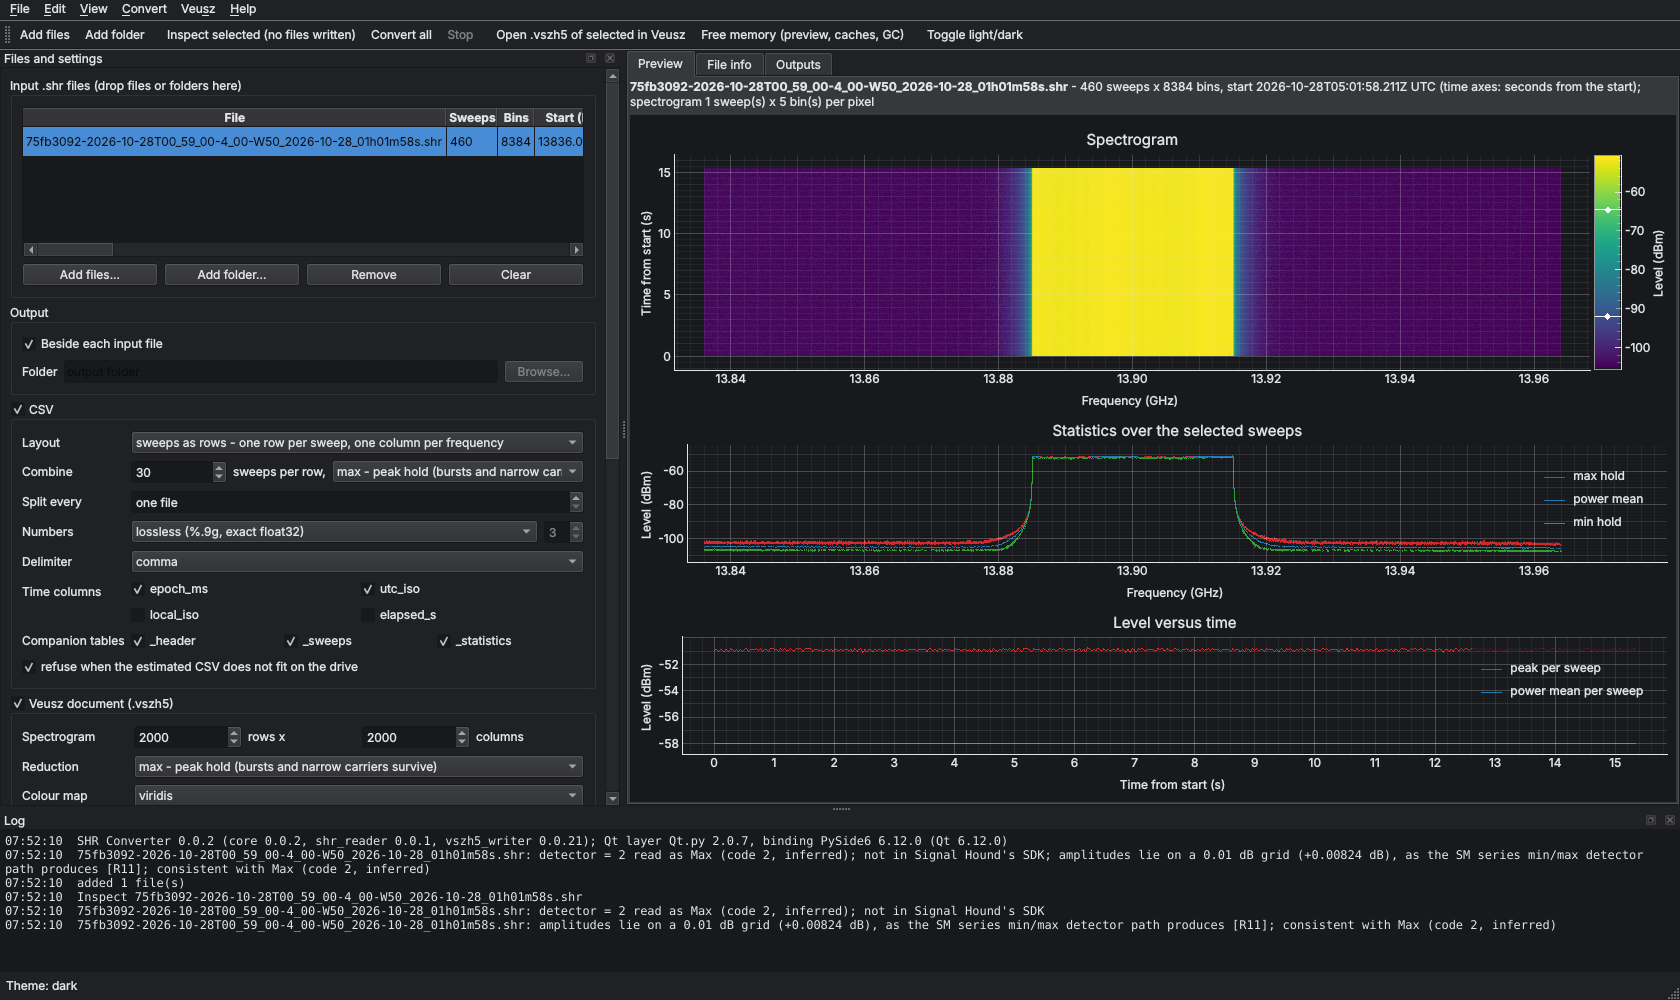
\includegraphics[width=\linewidth]{figures/gui_dark.png}
\caption{Dark theme, a synthetic 3-hour capture inspected: input list and settings (left), preview (centre), log (bottom).}
\end{figure}
\begin{figure}[htbp]\centering
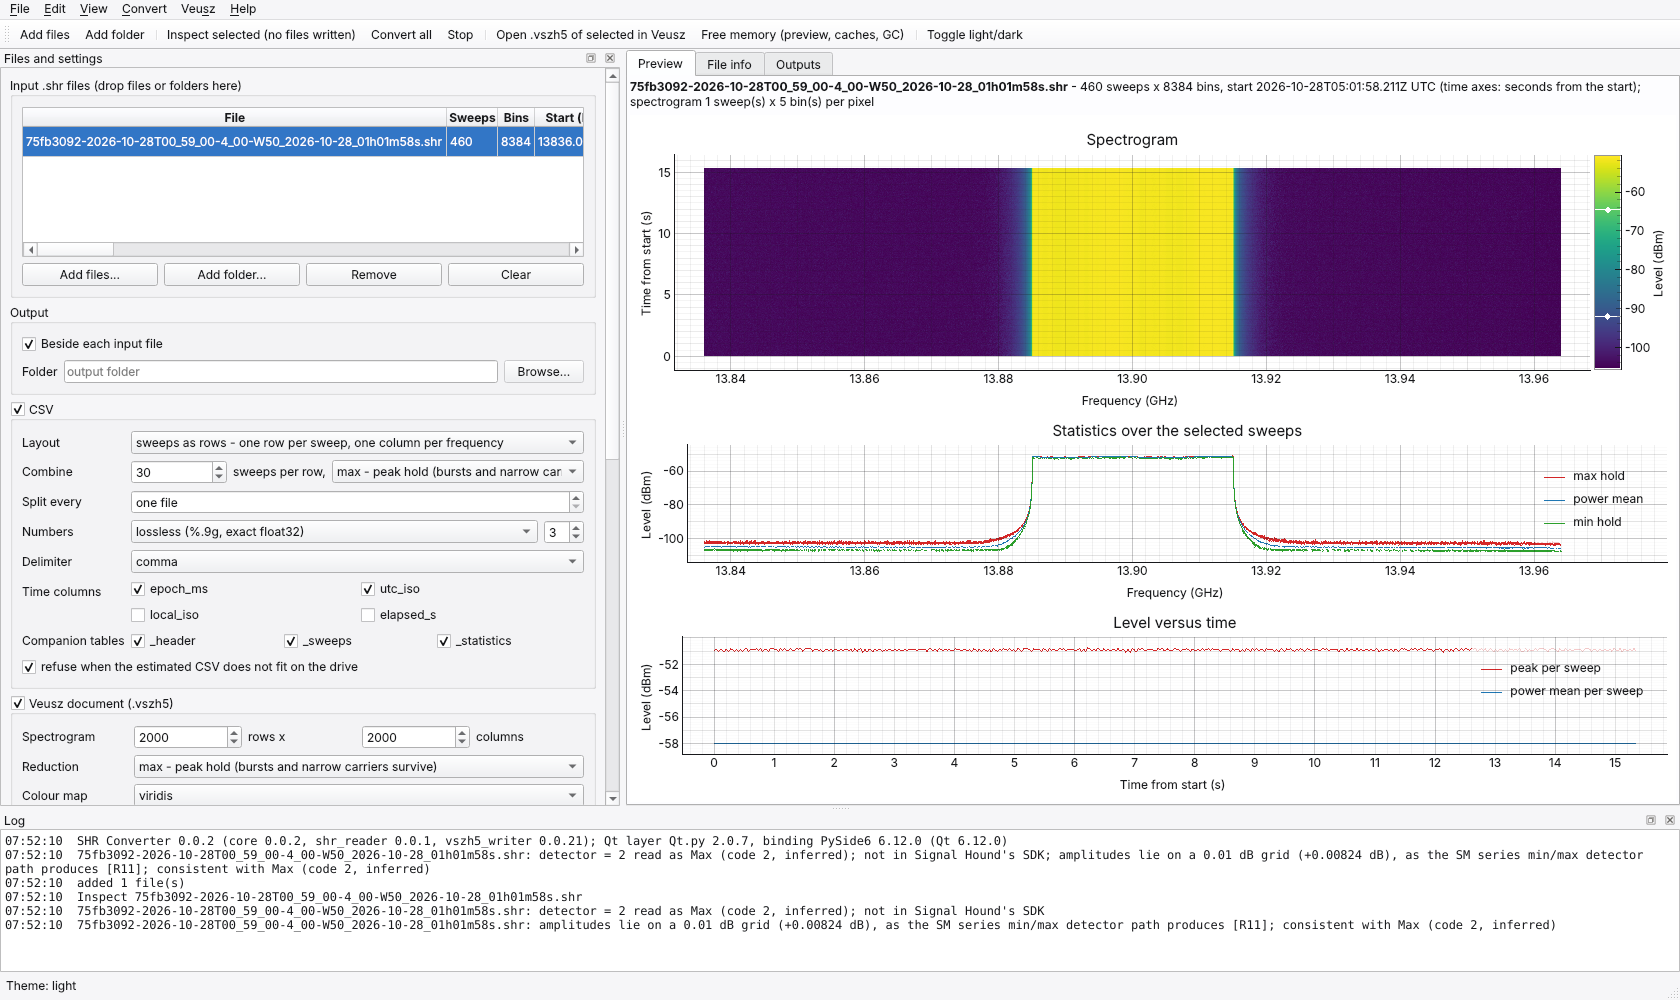
\includegraphics[width=\linewidth]{figures/gui_light.png}
\caption{Light theme (View > Theme, or Ctrl+T to toggle).}
\end{figure}
\subsection{Menus and keys}
\begin{description}[nosep,leftmargin=2.2cm,style=nextline]
\item[File] Add files (Ctrl+O), Add folder (Ctrl+Shift+O), Recent inputs, Remove (Del), Clear, Output folder,
      Open output folder (Ctrl+Shift+D), Save/Load settings (JSON), Save log, Quit.
\item[Edit] Copy file info, copy/clear log, \textbf{Free memory} (Ctrl+Shift+M).
\item[View] \textbf{Theme: System / Light / Dark}, toggle light/dark (Ctrl+T), auto-range (Ctrl+0), panels,
      toolbar, full screen (F11).
\item[Convert] Inspect (Ctrl+I), Convert all (F5), Convert selected (Shift+F5), Stop (Esc), Show plan (Ctrl+P),
      Self-test.
\item[Veusz] Open the \code{.vszh5} in Veusz (Ctrl+Shift+Z), Render to PDF/PNG (Ctrl+R), Open PDF.
\item[Help] Manual (F1), keyboard shortcuts, About (author, licence, every loaded version), About Qt.
\end{description}
\subsection{Workflow}
\begin{enumerate}[nosep]
\item Add files. Each header is read at once (sweeps, bins, span, length, detector); notes report cut-short
      recordings, unknown codes and the 0.01~dB grid.
\item Settings: \emph{CSV > Combine N sweeps per row} with its detector (Section~\ref{sec:decimate});
      \emph{Selection > Join the files of one recording} (Section~\ref{sec:join}).
\item \textbf{Inspect} runs the complete statistics pass without writing any file --- the same code as
      Convert --- and shows the preview. The \emph{File info} tab shows the plan (Figure~\ref{fig:info}).
\item \textbf{Convert}: one worker pool serves the whole batch; each file's preview arrives when it is
      done. \textbf{Stop} ends after the current block and deletes that file's partial outputs. Every file
      of a joined recording shows its status.
\end{enumerate}
\begin{figure}[htbp]\centering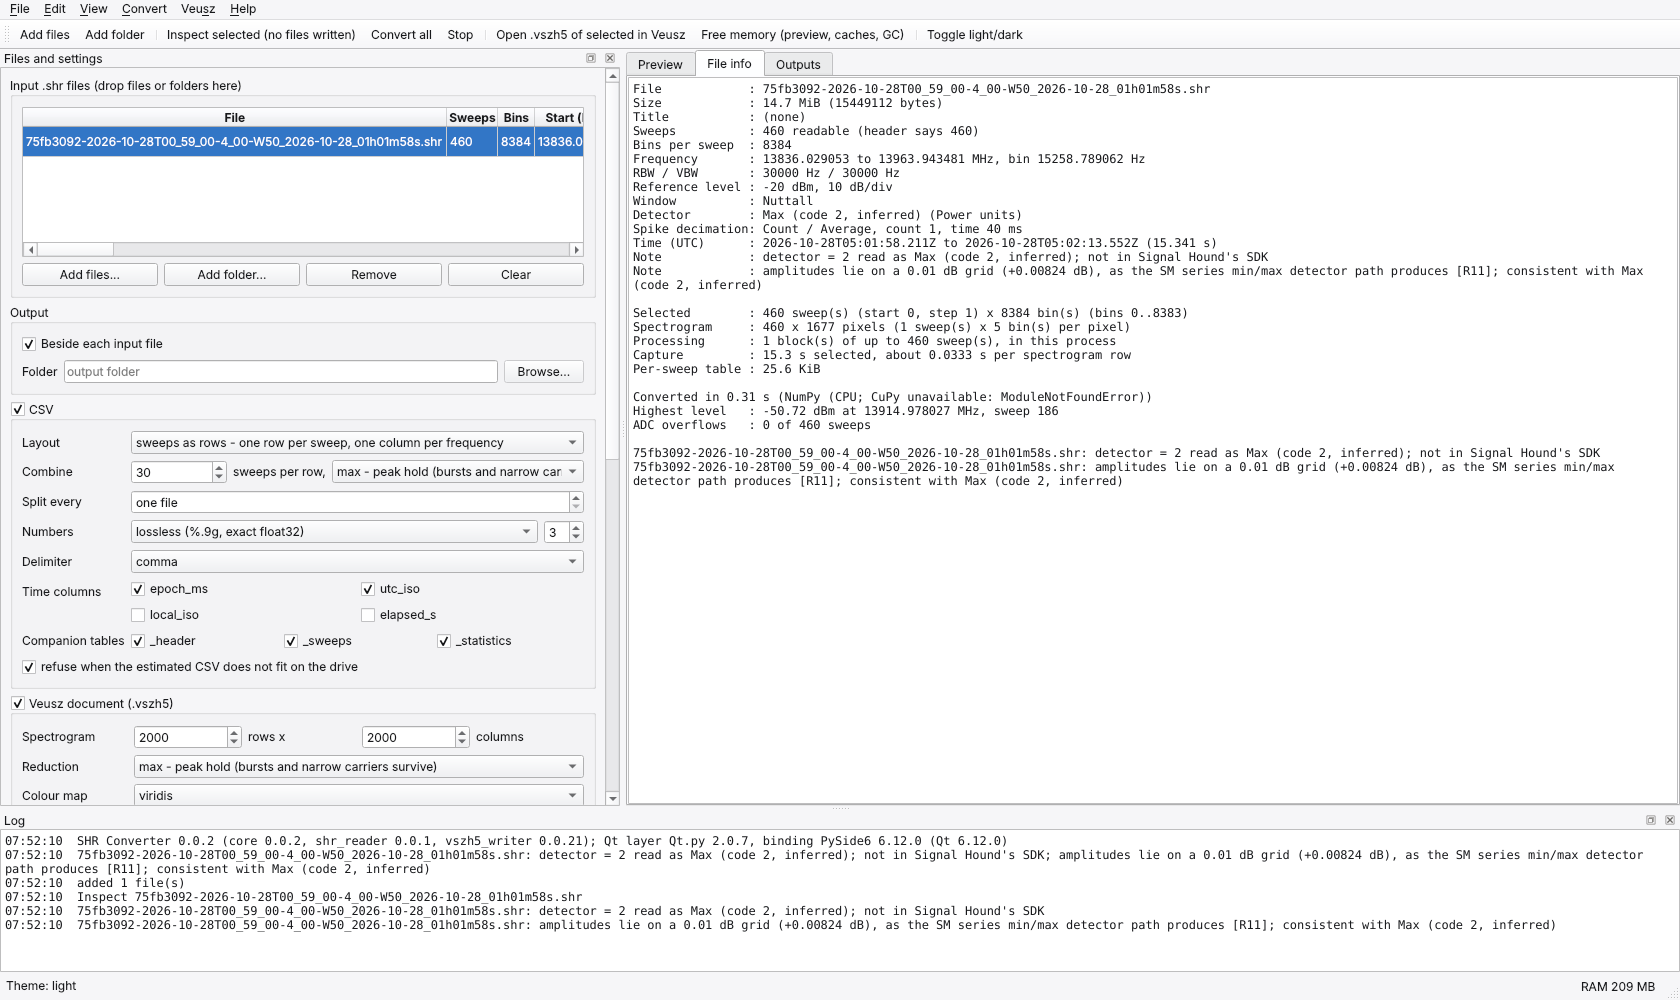
\includegraphics[width=\linewidth]{figures/gui_fileinfo.png}
\caption{File info: header, plan, CSV estimate, seconds per spectrogram row and free disk space.}\label{fig:info}
\end{figure}

\section{Outputs}
\subsection{CSV}
\begin{description}[nosep,leftmargin=3.6cm,style=nextline]
\item[\code{sweeps\_as\_rows}] one row per sweep: index, time columns, GPS, overflow, then one column per
      frequency (header: the bin frequencies in Hz). The default.
\item[\code{frequencies\_as\_rows}] one row per bin: frequency, then one column per sweep. Needs every
      selected sweep of a column block at once, so the file is read once per block (the plan says how often).
\item[\code{long}] one row per sample: index, time columns, frequency, amplitude.
\end{description}
With \code{csv\_decimate} $>1$ a \code{sweeps\_combined} column follows the time columns. Companion
tables: \code{\_header.csv} (every header field with its unit and enumeration label, derived values, CSV parts
with their time spans, the files of a joined recording, versions), \code{\_sweeps.csv} (per sweep: time,
GPS, overflow, peak, peak frequency, power mean) and \code{\_statistics.csv} (per bin: max hold, min hold,
power mean, dB mean, standard deviation, count). Files are written to private \code{.part} names and
published only when complete; a CSV that another program holds open (Excel on Windows) is kept under a
time-stamped name. Excel's limits (16\,384 columns, 1\,048\,576 rows \cite{r6}) are reported by the plan.

\subsection{Veusz document}
\begin{longtable}{ll}
\toprule
\textbf{Page} & \textbf{Title (PDF bookmark)}\\
\midrule
\endhead
\texttt{spectrogram} & Spectrogram\\
\texttt{statistics} & Spectrum statistics\\
\texttt{selected\_\allowbreak{}sweeps} & Selected sweeps\\
\texttt{level\_\allowbreak{}vs\_\allowbreak{}time} & Level versus time\\
\texttt{gps\_\allowbreak{}track} & GPS track\\
\texttt{file\_\allowbreak{}header} & File header\\
\bottomrule
\end{longtable}
\begin{figure}[htbp]\centering
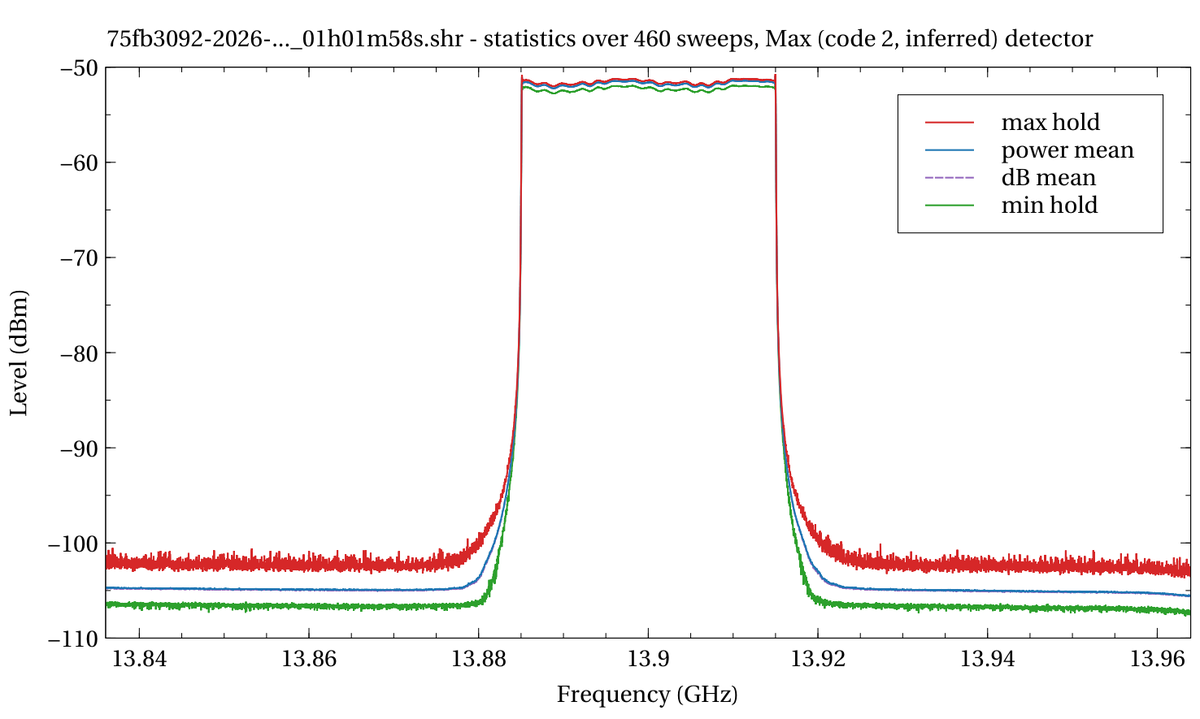
\includegraphics[width=\linewidth]{figures/veusz_statistics_sm200c.png}
\caption{Statistics page of the SM200C sample (460 sweeps, detector code 2 shown as Max, inferred); frequency axis in GHz.}
\end{figure}
\begin{figure}[htbp]\centering
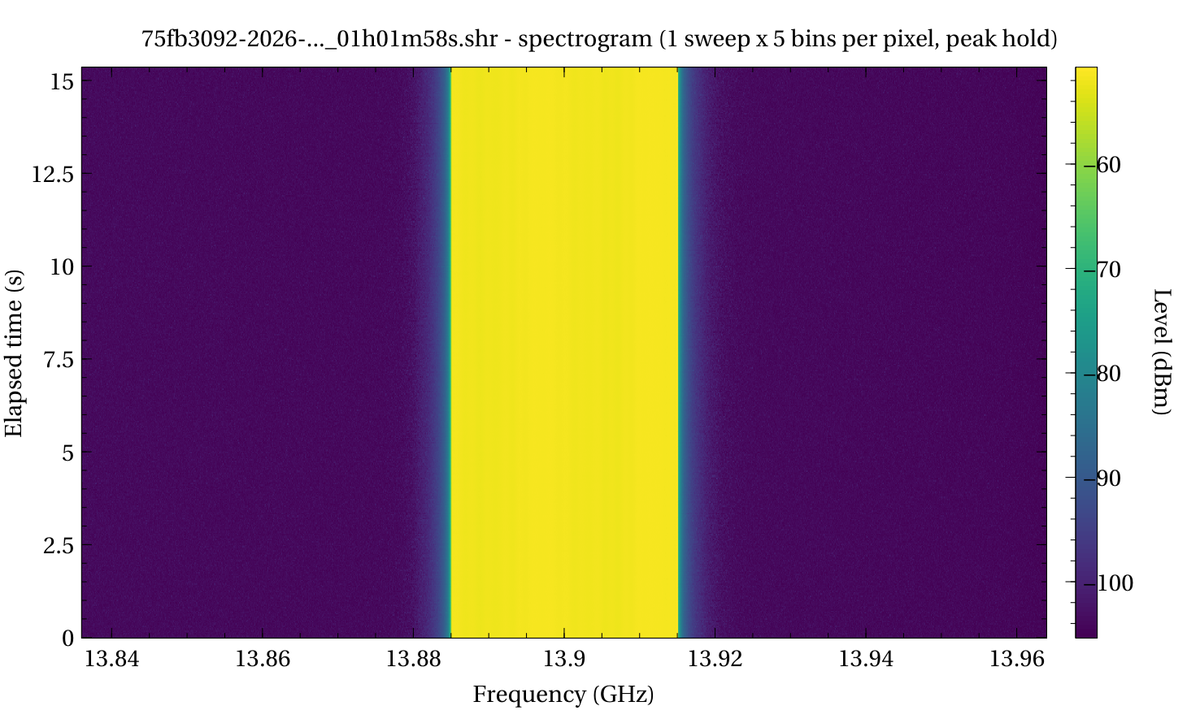
\includegraphics[width=\linewidth]{figures/veusz_spectrogram_sm200c.png}
\caption{Spectrogram page of the SM200C sample: every row present (no false blank rows with writer 0.0.21).}
\end{figure}
\begin{figure}[htbp]\centering
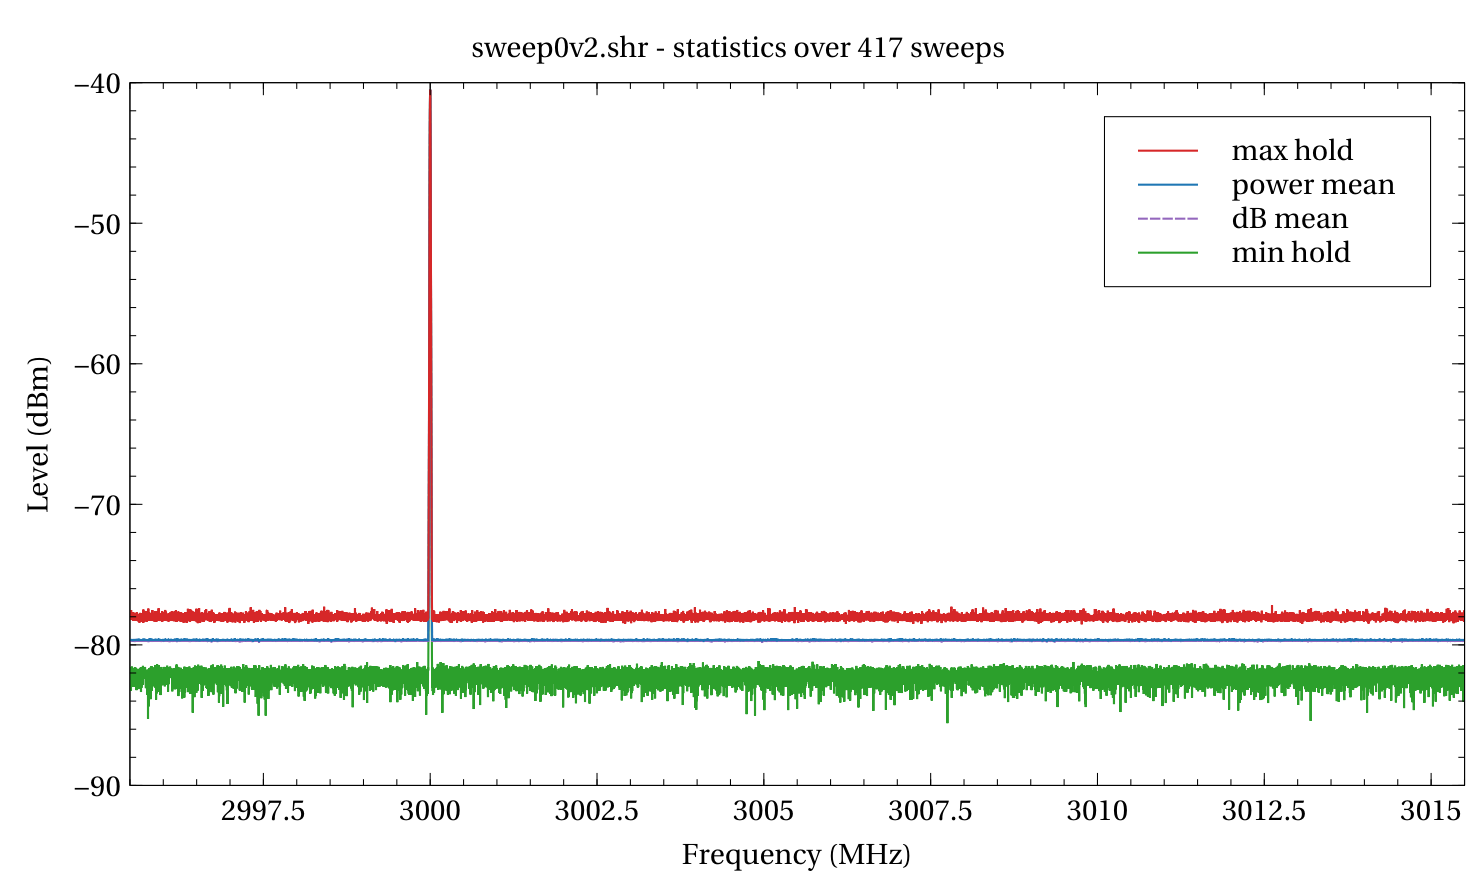
\includegraphics[width=\linewidth]{figures/veusz_statistics_sweep0v2.png}
\caption{Statistics page of Spike's own test file sweep0v2.shr (417 sweeps): max hold, power mean, dB mean, min hold.}
\end{figure}

\section{Multi-file recordings}\label{sec:join}
Since Spike~3.9.7 a long recording continues in a new, sequentially numbered file when the maximum file size is
reached \cite{r9},\cite{r12}. The naming scheme is not documented, so \code{group\_recordings} groups files by
content:
\begin{enumerate}[nosep]
\item Files are sorted by their first time stamp.
\item A file joins the previous group when these fields are equal: \texttt{sweep\_\allowbreak{}length}, \texttt{first\_\allowbreak{}bin\_\allowbreak{}freq\_\allowbreak{}hz}, \texttt{bin\_\allowbreak{}size\_\allowbreak{}hz}, \texttt{ref\_\allowbreak{}scale}.
\item and it starts no later than
      \begin{equation}t_\mathrm{first}^{(j)}-t_\mathrm{last}^{(j-1)}\le\max\big(10~\mathrm s,\ 50\,\tilde\Delta\big),\end{equation}
      $\tilde\Delta$ being the median sweep interval of the previous file.
\item Differences in \texttt{center\_\allowbreak{}freq\_\allowbreak{}hz}, \texttt{span\_\allowbreak{}hz}, \texttt{rbw\_\allowbreak{}hz}, \texttt{vbw\_\allowbreak{}hz}, \texttt{detector}, \texttt{processing\_\allowbreak{}units}, \texttt{window}, \texttt{ref\_\allowbreak{}level}, \texttt{attenuation}, \texttt{gain}, \texttt{decimation\_\allowbreak{}type}, \texttt{decimation\_\allowbreak{}detector}, \texttt{decimation\_\allowbreak{}count}, \texttt{decimation\_\allowbreak{}time\_\allowbreak{}ms}, \texttt{channelize\_\allowbreak{}enabled}, \texttt{channel\_\allowbreak{}output\_\allowbreak{}units} are reported, not refused.
\end{enumerate}
A \code{ShrFileSet} numbers the sweeps of $J$ files continuously: with $N_i$ sweeps in file $i$, sweep $k_j$ of
file $j$ has the recording-wide index
\begin{equation}k=O_j+k_j,\qquad O_j=\sum_{i<j}N_i ,\end{equation}
and a read that crosses a file boundary is split and joined transparently. Outputs are named
\code{<first file>\_joined.*}; \code{\_header.csv} lists every source file, and gaps between files are noted.
Files that do not group are converted on their own (\code{--join} with \code{--info} shows the grouping).

\section{CSV time decimation}\label{sec:decimate}
At the SM200C sample's rate a 3-hour recording is about 10.1 GiB of \code{.shr};
lossless CSV needs about 12 bytes per value, so roughly three times as much. \code{csv\_decimate} $=N$
combines every $N$ selected sweeps into one CSV row (one column in the \code{frequencies\_as\_rows} layout).
With $G_r$ the sweeps of row $r$ (blocks aligned to multiples of $N$; the last group may be shorter):
\begin{align}
y^{\max}_r(f)&=\max_{k\in G_r}x_k(f), \qquad y^{\min}_r(f)=\min_{k\in G_r}x_k(f),\\
y^{P}_r(f)&=10\log_{10}\Big(\frac{1}{|G_r|}\sum_{k\in G_r}10^{x_k(f)/10}\Big)\quad[\mathrm{dBm}],
\qquad y^{V}_r(f)=\sqrt{\frac{1}{|G_r|}\sum_{k\in G_r}x_k(f)^2}\quad[\mathrm{mV}].
\end{align}
\begin{longtable}{lp{10cm}}
\toprule
\textbf{Detector} & \textbf{Use}\\
\midrule
\endhead
\texttt{max} & peak hold (bursts and narrow carriers survive)\\
\texttt{power\_\allowbreak{}mean} & power mean (linear power, or RMS for mV)\\
\texttt{min} & minimum hold (noise floor)\\
\bottomrule
\end{longtable}
Each row carries the index, time stamp and GPS fix of the \emph{first} sweep of its group, ADC overflow if any
sweep of the group overflowed, and $|G_r|$ in \code{sweeps\_combined}. Only the main CSV is decimated: the
statistics, the spectrogram, \code{\_sweeps.csv} and the \code{.vszh5} always use every selected sweep.
\begin{longtable}{rrrr}
\caption{A 3-hour recording at 29.92 sweeps/s x 8384 bins (the SM200C sample's settings), sweeps\_as\_rows.}\\
\toprule
\textbf{N} & \textbf{CSV rows} & \textbf{Time per row} & \textbf{Lossless CSV (estimate)}\\
\midrule
\endhead
1 & 323,134 & 0.03 s & 30.3 GiB\\
10 & 32,314 & 0.33 s & 3.0 GiB\\
30 & 10,772 & 1.00 s & 1.0 GiB\\
300 & 1,078 & 10.03 s & 103.7 MiB\\
\bottomrule
\end{longtable}

\section{Statistics and their derivations}
Let $x_k(f)$ be the level of bin $f$ in sweep $k$, $k=1\ldots N$.
\subsection{Frequency of a bin}
\begin{equation}f_i = f_0 + i\,\Delta f,\qquad f_0=\code{firstBinFreqHz},\ \Delta f=\code{binSizeHz},\end{equation}
as the SDK defines the bin axis \cite{r1}.
py-shr-parser's plotting helpers \cite{r10} use $\mathrm{linspace}(f_c-S/2, f_c+S/2, n)$ instead; on
\code{sweep0v2.shr} ($\Delta f = 1220.703125$~Hz, $n=16\,386$, $S=20$~MHz) the two differ by up to one bin at
the top, because $(n-1)\,\Delta f = 20.0012$~MHz $\neq S$. Frequency axes switch to GHz from 10~GHz up, before
Veusz would print scientific tick labels.
\subsection{Power mean, dB mean and the 2.51 dB bias}
\begin{align}
\bar P(f) &= 10\log_{10}\!\Big(\frac1N\sum_{k=1}^{N}10^{x_k(f)/10}\Big)\quad[\mathrm{dBm}],\\
\bar L(f) &= \frac1N\sum_{k=1}^{N}x_k(f)\quad[\mathrm{dBm}].
\end{align}
For noise the dB mean reads low \cite{r4},\cite{r13}. With a Rayleigh envelope the power $p$ is exponential
with mean $\mu$, $\rho(p)=\mu^{-1}e^{-p/\mu}$, and with $u=p/\mu$
\begin{equation}
\mathrm{E}[\ln p]=\ln\mu+\int_0^\infty \ln u\,e^{-u}\,\mathrm du=\ln\mu+\Gamma'(1)=\ln\mu-\gamma,
\end{equation}
so
\begin{equation}
\mathrm{E}[10\log_{10}p]-10\log_{10}\mu=-\frac{10\,\gamma}{\ln 10}=-2.5068~\mathrm{dB},
\qquad \gamma=0.5772156649\ldots
\end{equation}
(a $10^7$-sample simulation gave $-2.5067$~dB). The converter therefore reports both: the power mean is the
physical mean power, the dB mean matches Spike's log averaging. With a Max detector each $x_k$ is already a
maximum over many FFTs (Section~\ref{sec:format}), so these statistics describe the recorded max-hold traces.
\subsection{mV recordings}
\begin{equation}V_\mathrm{rms}(f)=\sqrt{\frac1N\sum_k x_k(f)^2}\quad[\mathrm{mV}].\end{equation}
\subsection{Standard deviation from running sums}
\begin{equation}s^2=\frac{S_2-S_1^2/N}{N-1},\qquad S_1=\sum_k x_k,\ S_2=\sum_k x_k^2 .\end{equation}
In float64 the cancellation error is about $\varepsilon\,\bar x^2/s^2\approx 10^{-16}\times 80^2/2^2\approx
2\times10^{-13}$ (relative), negligible for dBm levels.
\subsection{Exact merging of blocks}
Each block returns $\max$, $\min$, $S_1$, $S_2$, $\sum 10^{x/10}$ and $N$ per bin; the file's values follow
exactly: maxima of maxima, minima of minima, sums of sums, e.g.
$\bar P_{A\cup B}=10\log_{10}\big((\Sigma_A+\Sigma_B)/(N_A+N_B)\big)$. Parallel and serial conversions give
identical results (self-test).
\subsection{Spectrogram pixels}
A pixel covers $n_r$ sweeps $\times$ $n_c$ bins. Peak hold is the block maximum; the power mean is
\begin{equation}
\bar P_{ij}=10\log_{10}\Big(\frac{1}{n_r n_c}\sum_{k\in r_i}\sum_{f\in c_j}10^{x_k(f)/10}\Big)
=10\log_{10}\Big(\frac{1}{n_r}\sum_{k\in r_i}\Big[\frac1{n_c}\sum_{f\in c_j}10^{x_k(f)/10}\Big]\Big),
\end{equation}
computed as the column mean per sweep, then summed over the sweeps of the row (exact, since every sweep of a
row has the same $n_c$). A row may span two worker blocks; its partial sums are added by the main process.
\subsection{Lossless numbers}
Binary32 has $p=24$ significand bits; a decimal string round-trips with \cite{r5},\cite{r16}
\begin{equation}d=\lceil p\log_{10}2\rceil+1=\lceil 7.22\rceil+1=9\end{equation}
significant digits, hence \code{\%.9g}. Every value of every layout was compared with the file's float32
values bit for bit (and with py-shr-parser \cite{r10} on \code{sweep0v2.shr}, which it can read).

\section{Time axes and the even grid}\label{sec:grid}
Time stamps are whole milliseconds since 1970 UTC from the recording PC's clock \cite{r2}. The \code{.vszh5}
time axis is UTC or local date/time, elapsed seconds or sweep index (\code{auto}: date/time for captures of
60~s or more). Veusz draws images with uneven axes through a slow non-linear path (on a 3-hour spectrogram
30.3~s and 3.2~GB, against 2.7~s and 0.31~GB on an even grid), so the rows are put on an even grid by
\code{vszh5\_writer.regularize\_rows} (0.0.21). With row centres $c_k$, intervals
$d_k=c_{k+1}-c_k$, median $\tilde d$ and tolerance $\tau=0.25$:
\begin{align}
\text{ordinary}_k &: d_k\le(1+2\tau)\,\tilde d,\qquad
\Delta=\operatorname{mean}\{d_k:\text{ordinary}_k\},\\
s_0&=0,\qquad s_{k+1}=s_k+\begin{cases}1 & \text{ordinary}_k\\ \max\!\big(1,\operatorname{rint}(d_k/\Delta)\big) & \text{otherwise}\end{cases}
\end{align}
Row $k$ goes to slot $s_k$; empty slots are blank (NaN) rows and show a pause. Why the mean: a step $\Delta'$
that differs from the true mean interval $\mu$ advances each row by $\mu/\Delta'$ slots, so the rounding skips a
slot about every $\Delta'/|\mu-\Delta'|$ rows. Spike's whole-millisecond stamps make the SM200C intervals
32--35~ms (mean 33.35~ms, median 33~ms); version 0.0.20, which took its step from the median, left a false blank
row about every 47 sweeps. With the mean of the ordinary intervals no slot is skipped, and a real 2-s pause
still gives 60 blank rows. Rows that are not strictly increasing are spread evenly instead (times approximate).

\section{Long captures}
\begin{itemize}[nosep]
\item \textbf{CSV split by time}: \code{\_part001.csv}, \ldots, one per N minutes of recording, each with the
      header line; slices follow the running maximum of the time stamps, so a clock step back never sends a
      sweep to an earlier file (and the step is noted).
\item \textbf{CSV decimation} (Section~\ref{sec:decimate}) and \textbf{joined files} (Section~\ref{sec:join}).
\item \textbf{Disk check}: the CSV size is estimated and the conversion refuses to start when the drive cannot
      hold it.
\item \textbf{Per-sweep table}: 57 bytes per sweep, memory-mapped from a private temporary folder when larger
      than a quarter of the RAM budget.
\item \textbf{Thinned series}: level versus time and GPS in the \code{.vszh5} are reduced to
      \code{time\_series\_max\_points} (100\,000) --- peak hold for the peak, power mean for the band level,
      the frequency of the strongest sweep, any overflow --- so a single burst is never averaged away.
\item \textbf{Time per row}: 2000 rows over 3~h is 5.4~s per row; the plan states it.
\end{itemize}
\begin{figure}[htbp]\centering
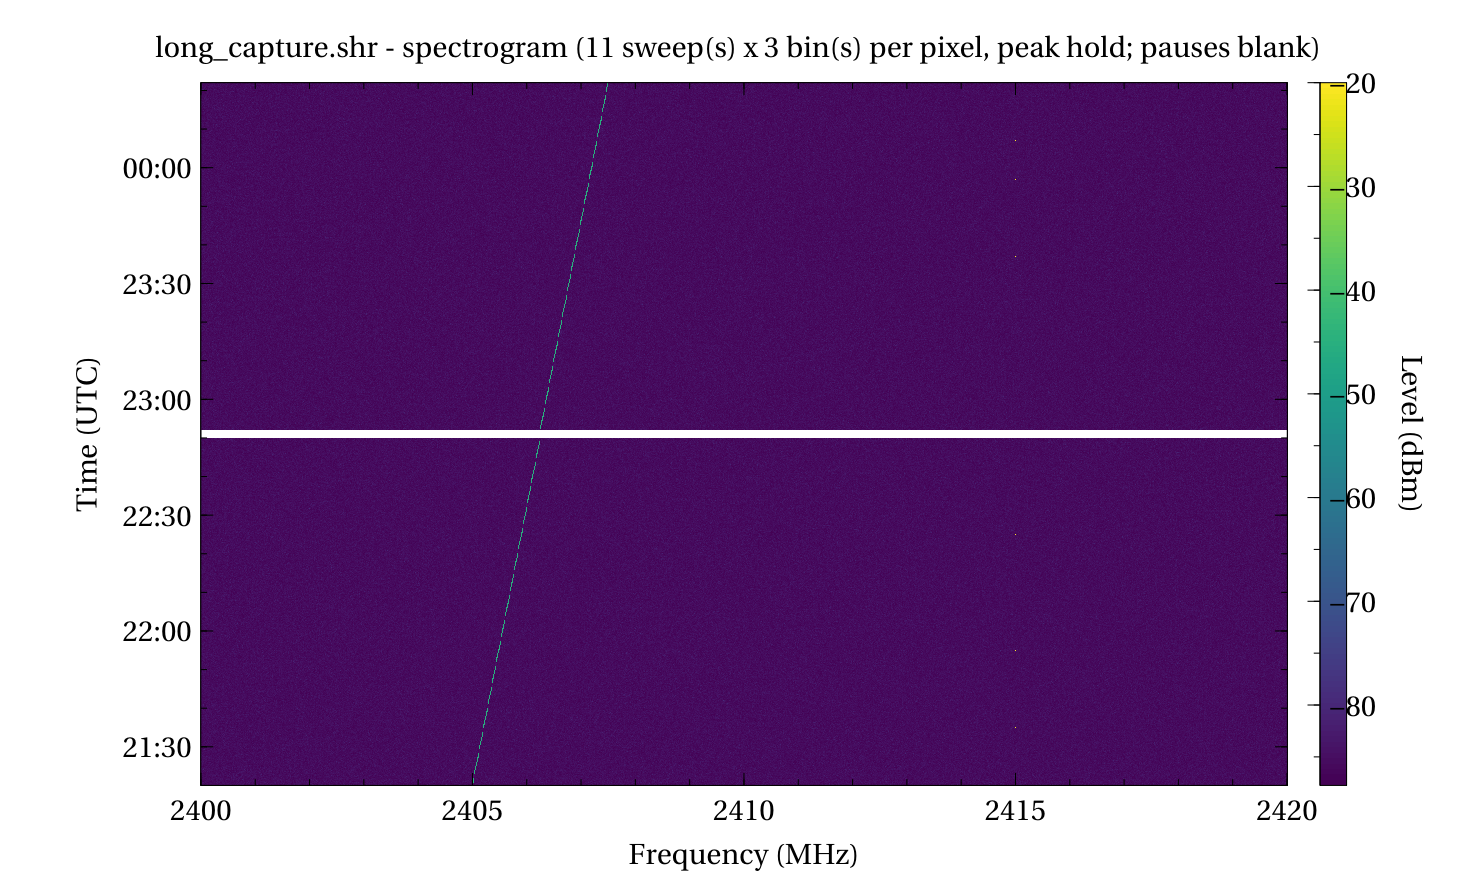
\includegraphics[width=\linewidth]{figures/veusz_spectrogram_3h.png}
\caption{Synthetic 3-hour capture: drifting carrier, a 2 ms burst every 10 min at 2415 MHz, a 2-minute pause (blank band).}
\end{figure}
\begin{figure}[htbp]\centering
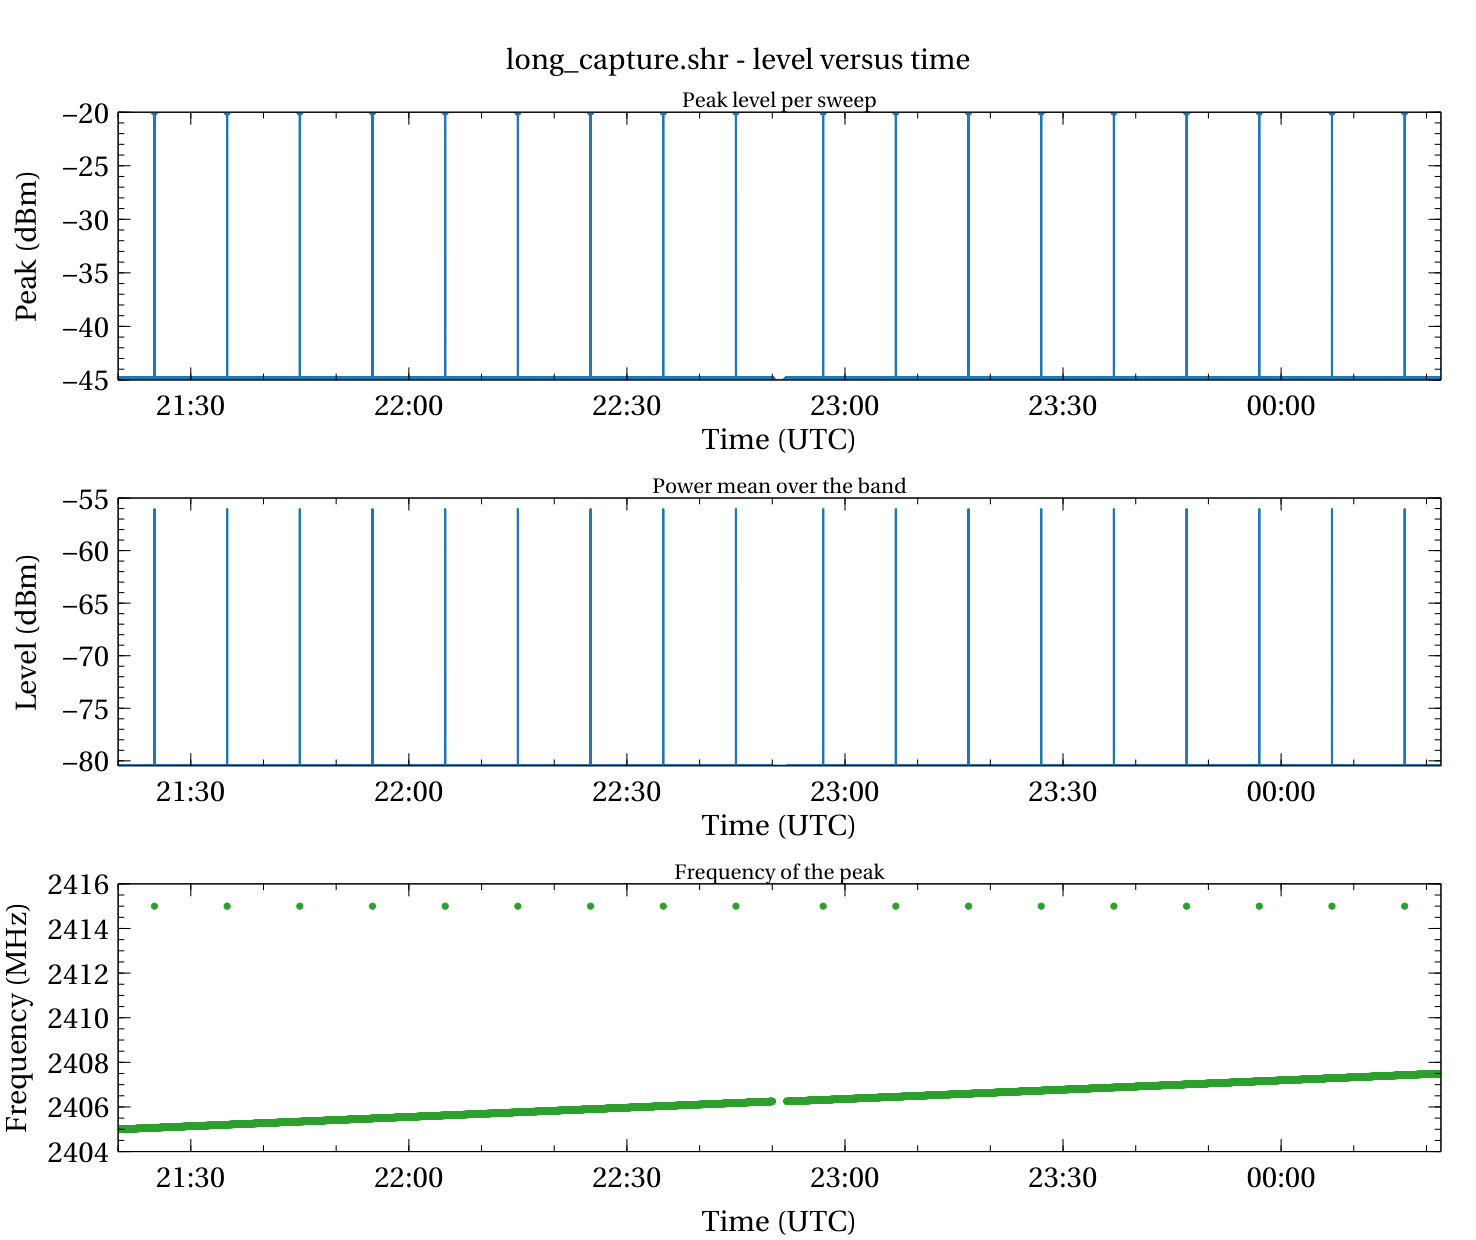
\includegraphics[width=\linewidth]{figures/veusz_level_vs_time_3h.png}
\caption{Level versus time of the same capture: every burst present, the pause visible.}
\end{figure}

\section{Performance, parallelism, GPU and memory}
\begin{itemize}[nosep]
\item Blocks of sweeps are read (one memory-mapped slice each), formatted and reduced in worker processes
      (\emph{spawn}, never fork a GUI), at most $2\times$workers blocks in flight, merged in order \cite{r7}.
      Default workers: CPUs $-1$ (at most 61 on Windows).
\item Block size: $B=\lfloor (M-M_\mathrm{stats})/(s\,n_c\,\beta)\rfloor$ with budget $M$, $s=2w+1$ slots,
      $n_c$ bins and $\beta$ bytes per sample in flight (30 for \code{sweeps\_as\_rows}); the statistics
      work in sub-blocks of 2~M samples, so their float64 temporaries do not grow with the block. With
      \code{csv\_decimate} $=N$, $B$ is rounded down to a multiple of $N$.
\item GPU: CuPy \cite{r8} runs the statistics and spectrogram reduction per sub-block; any GPU error repeats
      the block on the CPU (tested with a stand-in). Text formatting stays on the CPU.
\item Edit $>$ Free memory: garbage collection, CuPy pools, \code{malloc\_trim} / \code{EmptyWorkingSet};
      previews are pickled to disk, one in memory.
\end{itemize}
\begin{longtable}{p{6.2cm}p{4.2cm}rr}
\caption{Measured with tests/long\_capture\_check.py, tests/memory\_check.py and tests/sm200c\_rate\_check.py (docs/validation).}\\
\toprule
\textbf{Case (2 CPU cores, no GPU)} & \textbf{Data} & \textbf{Time} & \textbf{Peak memory}\\
\midrule
\endhead
3 h, 2 sweeps/s x 4001 bins, 1.5 ms jitter, 2 workers, with the Veusz PDF/PNG render & 331 MiB to 981 MiB CSV, 7 files & 27.9 s & 865 MiB\\
3 h, 50 sweeps/s x 512 bins (540 000 sweeps), 2 workers & 1.1 GiB to 3.1 GiB CSV & 58.9 s & 560 MiB\\
3000 x 65 536 bins, RAM budget 256 MB, 2 workers & 375 MiB to 1.1 GiB CSV & 21.4 s & 417 MiB\\
SM200C rate: 2 joined files x 10 min (35 902 sweeps x 8384 bins), csv\_decimate 30, 2 workers & 1.1 GiB to 114 MiB CSV (100.5 MiB/s of SHR) & 11.4 s & 477 MiB\\
\bottomrule
\end{longtable}

\section{Robustness}
\begin{itemize}[nosep]
\item The reader's validation and salvage rules (Section~\ref{sec:format}) turn cut-short, unclosed or
      unusual files into notes instead of errors; unknown enumeration codes never stop a conversion.
\item Memory maps are closed explicitly after every block and file, so Windows can move or delete the input.
\item Every output is written to a private \code{.part} and published atomically; Stop, an error or a
      refused disk check leaves no partial file.
\item Published files get the usual permissions (writer fix of the 0600 mode, since 0.0.20).
\end{itemize}

\section{Command line}
\code{python shr\_converter.py --cli [options] files-or-folders}
\begin{longtable}{p{4.6cm}p{11cm}}
\toprule
\textbf{Option} & \textbf{Meaning}\\
\midrule
\endhead
\texttt{inputs} & .shr files or folders (folders: every *.shr inside)\\
\texttt{-o, --output-dir} & output folder (default: beside each input)\\
\texttt{--no-csv} & do not write the CSV files\\
\texttt{--layout} & CSV layout: sweeps\_as\_rows (default), frequencies\_as\_rows or long\\
\texttt{--fixed} & fixed decimals instead of lossless \%.9g\\
\texttt{--delimiter} & CSV delimiter: comma (default), semicolon or tab\\
\texttt{--time-columns} & comma list of epoch\_ms, utc\_iso, local\_iso, elapsed\_s\\
\texttt{--no-companions} & skip \_header/\_sweeps/\_statistics.csv\\
\texttt{--split-minutes} & new CSV file every N minutes of recording (0 = one file)\\
\texttt{--csv-decimate} & combine every N selected sweeps into one CSV row (1 = every sweep)\\
\texttt{--csv-decimate-detector} & how --csv-decimate combines sweeps: max (peak hold, default), power\_mean or min\\
\texttt{--join} & convert the files of a multi-file Spike recording as one (grouped by content)\\
\texttt{--no-disk-check} & do not refuse when the CSV may not fit\\
\texttt{--no-vszh5} & do not write the Veusz document\\
\texttt{--image-size} & maximum spectrogram ROWSxCOLUMNS\\
\texttt{--reduction} & spectrogram pixels: max (peak hold, default), power\_mean or min\\
\texttt{--colormap} & Veusz colour map, e.g. viridis, magma, heat\\
\texttt{--z} & data | reference | veusz | MIN,MAX\\
\texttt{--time-axis} & auto (date/time from 60 s on), utc, local, elapsed or index\\
\texttt{--sweeps-to-plot} & selected-sweeps page: first,last,peak and/or sweep indices\\
\texttt{--render} & render PDF (bookmarked) and PNG with Veusz\\
\texttt{--png} & PNG pages when rendering: first (default), all or none\\
\texttt{--veusz} & Veusz program (else VEUSZ\_EXE, PATH, usual folders)\\
\texttt{--sweeps} & sweep selection START:STOP:STEP (STOP exclusive)\\
\texttt{--freq} & frequency range FMIN:FMAX in MHz\\
\texttt{-j, --workers} & worker processes (0 = CPUs - 1)\\
\texttt{--ram-mb} & RAM budget for blocks\\
\texttt{--compute} & statistics on auto (CuPy GPU when present), cpu or gpu (falls back to CPU)\\
\texttt{--series-points} & maximum points of the level-vs-time and GPS series in the .vszh5\\
\texttt{--sweep-table} & per-sweep table in RAM or memory-mapped on disk (auto: by size)\\
\texttt{--info} & print header, plan and notes only\\
\texttt{--selftest} & run the self-test and exit\\
\texttt{--real-file} & also check this real .shr in the self-test\\
\texttt{--version} & show program's version number and exit\\
\bottomrule
\end{longtable}
Examples:
\begin{itemize}[nosep]
\item \code{python shr\_converter.py --cli --join --csv-decimate 30 D:\textbackslash{}captures} --- every
      recording in the folder, files of one recording joined, 30 sweeps per CSV row (peak hold).
\item \code{python shr\_converter.py --cli --info --join *.shr} --- headers, notes and the grouping only.
\item \code{python shr\_converter.py --reader --group *.shr} --- the reader's own view of the files.
\end{itemize}

\section{vszh5\_writer 0.0.21}
0.0.21 is 0.0.20 with one fix in \code{regularize\_rows()} (Section~\ref{sec:grid}); no public
name, parameter, position or default of 0.0.5, 0.0.10, both 0.0.18 releases, 0.0.19 or 0.0.20 changed. 0.0.20
had joined the two releases both numbered 0.0.18 (R\&S FSP logger 0.9.0: render fixes; AB Power Meter Monitor
1.6.0: \code{VeuszAppender}) with 0.0.19, and added the 0600 file-mode fix, \code{png\_background}, date-axis
images, \code{block\_reduce} and \code{regularize\_rows}. No other program calls \code{regularize\_rows()}.
\begin{longtable}{p{4.0cm}p{5.0cm}p{6.0cm}}
\caption{Details: docs/WRITER\_0.0.21\_NOTES.md and docs/validation/writer\_compatibility\_0.0.21.}\\
\toprule
\textbf{Program} & \textbf{Own suite with 0.0.21} & \textbf{Note}\\
\midrule
\endhead
R\&S FSP logger 0.9.0 & 44/44 (PySide6; Veusz 4.2.1) & set the About test's expected writer version to 0.0.21\\
AB Power Meter Monitor 1.7.0 & 45 PASS, 0 FAIL & none\\
SA Time Stability Tools 0.0.3 & 7/7 and 22/22 in Veusz 4.2.1 & none\\
QuickSyn package 0.0.10 & 44 pass, 3 pinned checks fail & same with 0.0.19 and 0.0.20: version literal and pre-0.0.15 temporary name\\
EMF Envelope FFT 0.0.4, RFI evaluator 0.0.5 & API check only & they use the 0.0.13/0.0.14 API, unchanged\\
\bottomrule
\end{longtable}

\section{Verification}
\code{shr\_reader.py --selftest}: 39 checks (header size and field offsets, write/read round trip
bit-exact, UTF-16 title, detector 2 and unknown codes kept with notes, versions 1 and 3, \code{dataOffset}
1024, salvage of unclosed and cut-short files, bad signature refused, file sets across boundaries, grouping,
pickling, 0.01~dB grid detection, time stamps going backwards). \code{--selftest}:
58 engine checks with a real file (every CSV layout bit-exact with 1 and 2 workers; statistics, spectrogram
and sub-block merging against direct NumPy; joins; decimation by all three detectors; cut-short files; mV; GPU
stand-in and fallback; split, disk check, disk-mapped table, thinning; locked file; cancel).
\code{--gui-smoke}: 12 offscreen GUI checks including real worker processes and a joined, decimated conversion.
\code{pytest tests}: 34 tests with 30 sub-tests, real renders in Veusz 4.2.1, Spike's own
\code{sweep0v2.shr} and the SM200C sample (shipped in \code{tests/data}). Logs: \code{docs/validation}.

\section{Data gaps}
\begin{longtable}{p{4.2cm}p{8.6cm}l}
\toprule
\textbf{Item} & \textbf{Status} & \textbf{Confidence}\\
\midrule
\endhead
Real Spike files & sweep0v2.shr (v2, dBm) and the SM200C sample (v2, detector 2) read bit-exactly & High\\
Detector code 2 = Max & inferred from the 0.01 dB grid and the noise shape; not in the SDK & Medium\\
Detector code 3 = Min & by analogy; no file seen & Low\\
MinMax (code 0) contents & which array a MinMax file stores is not known & Unknown\\
Multi-file recordings & grouped by content; Spike's naming not seen & Medium\\
Limit-line-triggered recordings & not seen; skipped sweeps would appear as pauses & Unknown\\
Channelized recordings & read as stored, not interpreted & Unknown\\
Spike time decimation & which instant a decimated sweep's time stamp marks is not known & Unknown\\
mV recordings & synthetic only & Medium\\
Title encoding & UTF-16LE per the SDK; no titled file seen & Medium\\
GPU & stand-in only; no CUDA device here & Medium\\
Windows & designed for it (spawn, explicit map close, locked CSV), tested on Linux & Medium\\
\bottomrule
\end{longtable}
The open format questions are in \code{docs/SignalHound\_support\_letter\_2026-10-28.md}.

\appendix
\section{Options (ConvertOptions) and their defaults}
\begin{longtable}{p{5.6cm}p{9.6cm}}
\toprule
\textbf{Field} & \textbf{Default}\\
\midrule
\endhead
\texttt{output\_\allowbreak{}dir} & \texttt{""}\\
\texttt{write\_\allowbreak{}csv} & \texttt{True}\\
\texttt{csv\_\allowbreak{}layout} & \texttt{"sweeps\_\allowbreak{}as\_\allowbreak{}rows"}\\
\texttt{csv\_\allowbreak{}number\_\allowbreak{}format} & \texttt{"lossless"}\\
\texttt{csv\_\allowbreak{}decimals} & \texttt{3}\\
\texttt{csv\_\allowbreak{}delimiter} & \texttt{"comma"}\\
\texttt{csv\_\allowbreak{}time\_\allowbreak{}columns} & \texttt{('epoch\_\allowbreak{}ms', 'utc\_\allowbreak{}iso')}\\
\texttt{csv\_\allowbreak{}header\_\allowbreak{}table} & \texttt{True}\\
\texttt{csv\_\allowbreak{}sweeps\_\allowbreak{}table} & \texttt{True}\\
\texttt{csv\_\allowbreak{}statistics\_\allowbreak{}table} & \texttt{True}\\
\texttt{csv\_\allowbreak{}split\_\allowbreak{}minutes} & \texttt{0.0}\\
\texttt{csv\_\allowbreak{}decimate} & \texttt{1}\\
\texttt{csv\_\allowbreak{}decimate\_\allowbreak{}detector} & \texttt{"max"}\\
\texttt{check\_\allowbreak{}disk\_\allowbreak{}space} & \texttt{True}\\
\texttt{write\_\allowbreak{}vszh5} & \texttt{True}\\
\texttt{vszh5\_\allowbreak{}compress} & \texttt{True}\\
\texttt{image\_\allowbreak{}max\_\allowbreak{}rows} & \texttt{2000}\\
\texttt{image\_\allowbreak{}max\_\allowbreak{}columns} & \texttt{2000}\\
\texttt{image\_\allowbreak{}reduction} & \texttt{"max"}\\
\texttt{colormap} & \texttt{"viridis"}\\
\texttt{z\_\allowbreak{}mode} & \texttt{"data"}\\
\texttt{z\_\allowbreak{}min} & \texttt{-120.0}\\
\texttt{z\_\allowbreak{}max} & \texttt{-20.0}\\
\texttt{time\_\allowbreak{}axis} & \texttt{"auto"}\\
\texttt{selected\_\allowbreak{}sweeps} & \texttt{"first,last,peak"}\\
\texttt{stats\_\allowbreak{}max\_\allowbreak{}points} & \texttt{200000}\\
\texttt{time\_\allowbreak{}series\_\allowbreak{}max\_\allowbreak{}points} & \texttt{100000}\\
\texttt{page\_\allowbreak{}spectrogram} & \texttt{True}\\
\texttt{page\_\allowbreak{}statistics} & \texttt{True}\\
\texttt{page\_\allowbreak{}selected\_\allowbreak{}sweeps} & \texttt{True}\\
\texttt{page\_\allowbreak{}level\_\allowbreak{}vs\_\allowbreak{}time} & \texttt{True}\\
\texttt{page\_\allowbreak{}gps} & \texttt{True}\\
\texttt{page\_\allowbreak{}header} & \texttt{True}\\
\texttt{render} & \texttt{False}\\
\texttt{render\_\allowbreak{}png} & \texttt{"first"}\\
\texttt{render\_\allowbreak{}dpi} & \texttt{150}\\
\texttt{veusz\_\allowbreak{}exe} & \texttt{""}\\
\texttt{sweep\_\allowbreak{}start} & \texttt{0}\\
\texttt{sweep\_\allowbreak{}stop} & \texttt{0}\\
\texttt{sweep\_\allowbreak{}step} & \texttt{1}\\
\texttt{freq\_\allowbreak{}min\_\allowbreak{}hz} & \texttt{0.0}\\
\texttt{freq\_\allowbreak{}max\_\allowbreak{}hz} & \texttt{0.0}\\
\texttt{join\_\allowbreak{}files} & \texttt{False}\\
\texttt{workers} & \texttt{0}\\
\texttt{ram\_\allowbreak{}budget\_\allowbreak{}mb} & \texttt{1024}\\
\texttt{compute} & \texttt{"auto"}\\
\texttt{sweep\_\allowbreak{}table\_\allowbreak{}storage} & \texttt{"auto"}\\
\texttt{flush\_\allowbreak{}after\_\allowbreak{}file} & \texttt{True}\\
\bottomrule
\end{longtable}
\section{File-header fields}
\begin{longtable}{p{4.4cm}p{2.2cm}p{8.6cm}}
\toprule
\textbf{Field} & \textbf{Unit} & \textbf{Meaning}\\
\midrule
\endhead
\texttt{signature} &  & file signature (0xAA10)\\
\texttt{version} &  & SHR format version\\
\texttt{data\_\allowbreak{}offset} & byte & offset of the first sweep\\
\texttt{sweep\_\allowbreak{}count} &  & sweeps according to the header\\
\texttt{sweep\_\allowbreak{}length} & bin & bins per sweep\\
\texttt{first\_\allowbreak{}bin\_\allowbreak{}freq\_\allowbreak{}hz} & Hz & frequency of bin 0\\
\texttt{bin\_\allowbreak{}size\_\allowbreak{}hz} & Hz & bin spacing\\
\texttt{center\_\allowbreak{}freq\_\allowbreak{}hz} & Hz & centre frequency\\
\texttt{span\_\allowbreak{}hz} & Hz & span\\
\texttt{rbw\_\allowbreak{}hz} & Hz & resolution bandwidth\\
\texttt{vbw\_\allowbreak{}hz} & Hz & video bandwidth\\
\texttt{ref\_\allowbreak{}level} & dBm or mV & reference level\\
\texttt{ref\_\allowbreak{}scale} &  & reference scale (dBm or mV)\\
\texttt{div} & dB & display division\\
\texttt{window} &  & RBW window\\
\texttt{attenuation} & dB & attenuation setting (as stored by Spike)\\
\texttt{gain} &  & gain setting (as stored by Spike)\\
\texttt{detector} &  & video detector (Max/Min codes are not in the SDK)\\
\texttt{processing\_\allowbreak{}units} &  & video processing units\\
\texttt{window\_\allowbreak{}bandwidth} & bin & window bandwidth in bins (RBW / bin spacing)\\
\texttt{decimation\_\allowbreak{}type} &  & time averaging type\\
\texttt{decimation\_\allowbreak{}detector} &  & time averaging detector\\
\texttt{decimation\_\allowbreak{}count} &  & sweeps per output trace (count decimation)\\
\texttt{decimation\_\allowbreak{}time\_\allowbreak{}ms} & ms & time averaging interval (time decimation)\\
\texttt{channelize\_\allowbreak{}enabled} &  & channelizer enabled (1) or not (0)\\
\texttt{channel\_\allowbreak{}output\_\allowbreak{}units} &  & channelizer units\\
\texttt{channel\_\allowbreak{}center\_\allowbreak{}hz} & Hz & channelizer centre\\
\texttt{channel\_\allowbreak{}width\_\allowbreak{}hz} & Hz & channelizer width\\
\bottomrule
\end{longtable}
\section{Modules and functions used, and why}
\begin{longtable}{p{3.8cm}p{5.2cm}p{6.4cm}}
\toprule
\textbf{Module} & \textbf{Used} & \textbf{Why}\\
\midrule
\endhead
\texttt{shr\_\allowbreak{}reader (0.0.1)} & ShrHeader, ShrFile, ShrFileSet, group\_recordings, detect\_amplitude\_grid & reads every header and sweep (memory-mapped, one vectorised read per block); picklable, so each worker opens its own map [1]\\
\texttt{struct} & Struct('\textless{}HHIQIIdd256s...64s') & the 472-byte file header in one call [1]\\
\texttt{numpy} & memmap with a structured dtype, float32/float64 arrays, ufunc.reduceat, add.reduceat, percentile & sweep records, statistics, block and CSV decimation, per-sweep table on disk\\
\texttt{cupy (optional)} & same array calls on the GPU & statistics and spectrogram reduction per sub-block [8]\\
\texttt{concurrent.futures} & ProcessPoolExecutor (spawn, max\_tasks\_per\_child) & parallel blocks, bounded and in order [7]\\
\texttt{h5py via vszh5\_\allowbreak{}writer} & VeuszWriter, image\_page, xy\_page, grid\_page, text\_page & native .vszh5 without Veusz\\
\texttt{vszh5\_\allowbreak{}writer (0.0.21)} & block\_reduce, regularize\_rows, render\_pages & thinning, even spectrogram grid, PDF/PNG with bookmarks [3]\\
\texttt{Qt.py + PySide6} & QtCore, QtGui, QtWidgets & the GUI through the abstraction layer [15]\\
\texttt{pyqtgraph} & ImageItem, ColorBarItem, PlotDataItem & preview plots\\
\texttt{psutil} & Process().memory\_info() & memory read-out and tests\\
\texttt{pypdf (via the writer)} & PdfWriter.add\_outline\_item & PDF bookmark tree\\
\texttt{ctypes} & malloc\_trim (Linux), EmptyWorkingSet (Windows) & return freed memory to the OS\\
\bottomrule
\end{longtable}

\section*{References}
\addcontentsline{toc}{section}{References}
\begin{thebibliography}{99}
\bibitem{r1} Signal Hound, ``SHR parsing example'' (\code{shr\_parse.h}, \code{shr\_parse.cpp}), in \emph{Signal Hound Software Development Kit}, release of 2026-10-05. \url{https://signalhound.com/software/signal-hound-software-development-kit-sdk/}
\bibitem{r2} Signal Hound, ``.shr file format specification,'' BB Series Discussions forum, May--Aug. 2018. \url{https://signalhound.com/?p=158701}
\bibitem{r3} W. W. Wallace, ``vszh5\_writer.py --- Veusz HDF5 document writer,'' v0.0.21, NRAO/GBO, 2026 (shipped with this program).
\bibitem{r4} Hewlett-Packard, ``Measuring Noise and Noise-like Digital Communications Signals with a Spectrum Analyzer,'' Application Note 1303, lit.\ no.\ 5966-4008E. \url{https://www.hpmemoryproject.org/an/pdf/an_1303.pdf}
\bibitem{r5} IEEE, ``IEEE Standard for Floating-Point Arithmetic,'' IEEE Std 754-2019, pp.~1--84, Jul. 2019, doi: 10.1109/IEEESTD.2019.8766229. \url{https://doi.org/10.1109/IEEESTD.2019.8766229}
\bibitem{r6} Microsoft, ``Excel specifications and limits.'' \url{https://support.microsoft.com/en-us/office/1672b34d-7043-467e-8e27-269d656771c3}
\bibitem{r7} Python Software Foundation, ``concurrent.futures --- Launching parallel tasks,'' Python 3.12. \url{https://docs.python.org/3.12/library/concurrent.futures.html}
\bibitem{r8} Preferred Networks, ``CuPy documentation.'' \url{https://docs.cupy.dev/}
\bibitem{r9} Signal Hound, ``Technical Software and Hardware Change Log'' (Spike), v4.0.17, Sep. 2026 (max/min detectors 3.5.7; multi-file sweep recording 3.9.7; limit-line triggered recording 4.0.17). \url{https://signalhound.com/sigdownloads/Spike/change_log.txt}
\bibitem{r10} T. Schmitz, ``py-shr-parser: Python library for parsing Signal Hound SHR files,'' v1.0.0, WiSE Lab, Carnegie Mellon Univ., 2025. \url{https://github.com/WiseLabCMU/py-shr-parser}
\bibitem{r11} Signal Hound, ``SM200A/B/C -- SM435B/C Product Manual,'' Jan. 2025 (min/max processing at 0.01~dB resolution). \url{https://signalhound.com/sigdownloads/SM200A/SM-User-Manual.pdf}
\bibitem{r12} Signal Hound, ``Spike Software Documentation'' (Sweep Record and Playback). \url{https://signalhound.com/sigdownloads/Spike/docs/html/index.html}
\bibitem{r13} Keysight Technologies, ``Spectrum Analysis Basics,'' Application Note 150, 5952-0292. \url{https://www.keysight.com/us/en/assets/7018-06714/application-notes/5952-0292.pdf}
\bibitem{r14} J. Sanders, ``Veusz --- a scientific plotting package.'' \url{https://veusz.github.io/}
\bibitem{r15} M. Ottosson \emph{et al.}, ``Qt.py,'' v2.0.7. \url{https://github.com/mottosso/Qt.py}
\bibitem{r16} R. Regan, ``Number of digits required for round-trip conversions,'' Exploring Binary. \url{https://www.exploringbinary.com/number-of-digits-required-for-round-trip-conversions/}
\end{thebibliography}
\end{document}
